\chapter{Relevant Background}
In this chapter we provide a brief overview of various concepts and useful information related to the thesis. In the following we first discuss what audio event detection is, followed by a brief description of neural networks in the machine learning context. Then, we discuss the previous related work and also introduce the concept of artificial data augmentation. We conclude this chapter by describing the audio datasets (set of recordings) that were used in the thesis work.

\section{Audio Event Detection}
An audio event detection system aims at detecting audio events in continuous audio recordings. Much of the previous research is done for isolated sound events \cite{gencoglu2014recognition}, where there is a single sound event in each recording and the audio event detection system is trained to detect an event occurring in a given time period. Such systems with one output audio event class per recording are called monophonic. If a single recording has more than one events, potentially overlapping with each other, then the audio event detection used in that case is polyphonic. In our thesis, we have worked on both monophonic and polyphonic systems. 

The entire process of audio event detection is carried out in various steps: pre-processing, feature-extraction, training and testing, which are discussed below:
\begin{enumerate}
\item \textbf{Pre-processing} Input audio data is preprocessed before being fed to the next stage i.e. feature extraction. General preprocessing operations include normalization, transformation, trimming, windowing, smoothing, etc. For e.g. in speech recognition systems, end-point detection is a common pre-processing step.
\item \textbf{Feature Extraction} Features are what is actually fed to the learning model as the input. Features are higher level representations compared to raw data, like frequencies instead of a raw temporal sample when using MFCCs for audio event detection. Features should be selected from the data in such a way that they contain enough information to properly represent the similarities between inter-class observations and variations between intra-class observations. In our work, MFCCs are the features that we extract from the audio recordings. \item \textbf{Training} Training phase in a machine learning model refers to the process of learning from labeled data. Audio event labels in a dataset are the audio event classes such as “Siren”, “Dog Barking”, “Gun Shot”, etc. that are annotated for each of the audio recordings. MFCC features are the inputs and labels are the output during the training of the machine learning model. Training a neural network, in particular, involves the computation of various hidden layers and non-linear transformations. Finally, the gradient back-propagates from the outermost layer to all the preceding hidden and input layer neurons. Details can be found at \cite{hastie2005elements}. \item \textbf{Testing} Once the model is trained, classification has to be performed on the test data i.e. the unseen data. The test data is completely isolated from the training data and represents the observations unseen to the system. The model’s performance by is judged by valuations done in this classification stage.
\end{enumerate}

There are quite a number of audio features that can be extracted from the audio recordings. The features are primarily spectral, spatial, compressive or low-level features. Table~\ref{tab:audio_feats} gives an overview of some commonly used features in audio tasks.

\begin{table}[tb]
\caption[Typical audio features]{Typical audio features}
\label{tab:audio_feats}
\centering
\begin{tabular}{ccc}
\toprule
Feature name	& Abbreviation & Category \\
\midrule
Mel Frequency Cepstrum Coefficients	& MFCC & Spectral\\
Gammatone Frequency Cepstrum Coefficients	& GFCC & Spectral \\
Zero Crossing Rate	& ZCR & Low-level descriptor \\
Low Energy Rate	& LER & Low-level descriptor \\
Spectral Centroid	& SC & Low-level descriptor \\
Spectral roll-off	& SRO & Low-level descriptor \\
Inter-aural time difference 	& ITD & Spatial \\
Inter-aural level difference & ILD & Spatial \\
Frequency band energy	& FBE & Spectral \\
Voicing	& N/A & Spectral \\
Linear Predictive Coding	& LPC & Compressive \\
\bottomrule 
\end{tabular}
\end{table}

The spectral features indicate how much of the input signal is found inside a certain frequency bands over a range of frequencies. Discrete Fourier Transforms (DFT) are used to convert temporal information to spectral by taking small windows or frames (10-100 milliseconds) of the audio signals and assuming the audio signal is stationary in that window. 

We have used MFCCs as our features. They are widely used in audio event recognition systems and are extremely effective in single source environments. These features are calculated by taking the log of mel-band energies and applying Discrete Cosine Transform(DCT). Logarithm is used for non-linearity because humans do not perceive loudness in audio in a linear scale. The MFCC extraction process is illustrated in figure~\ref{fig:mfcc_flow}.

\begin{figure}[!htb] 
\centering 
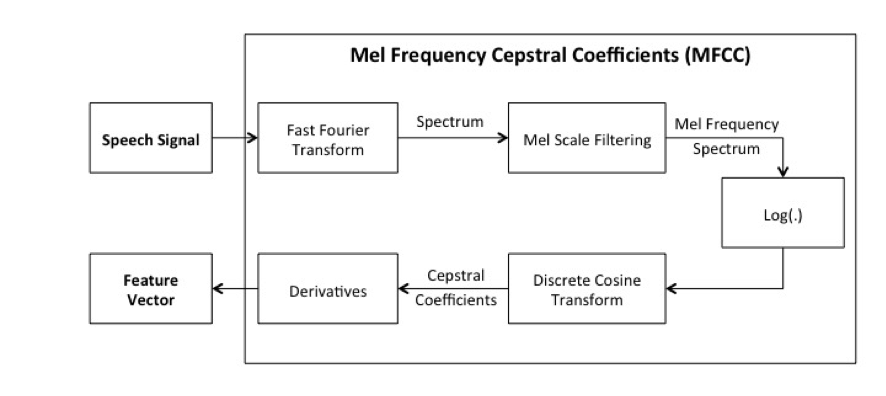
\includegraphics[width=0.95\columnwidth]{mfcc_flow}
\caption[MFCC Extraction Flowchart]{MFCC Extraction Flowchart}
\label{fig:mfcc_flow} 
\end{figure}

The most widely used classifiers in audio event detection are the GMM[13] and HMM[1]. Neural networks are now being increasingly used as well. We also use neural networks as our machine learning model for the audio event detection task and we discuss more about it in the next section.

\section{Neural Networks}

\section{Related work}

\section{Artificial (label-preserving) data augmentation}

\section{Datasets used}

The audio event detection task is subjective to the application and to the kind of audio recordings (data). There is no single defined taxonomy of sound events for which this task is to be performed. Different applications may demand different kinds of sound events, which in turn should have different kinds of audio recordings. For example, if the application of the audio event detection task is to determine if there is somebody (person) inside the house or not, then this puts a constraint that the audio recordings have to be from inside that house that we are talking about, and nowhere else. On the other hand, if the application is about identifying if there is too much traffic on the road, then no audio recordings taken inside any house would be of any help. Hence, the choice of the audio dataset (set of labeled recordings) is to be solely determined by the application we are aiming for. 

Another factor that could determine the kind of audio data set that is desired for the detection task, is whether the task is a monophonic audio event detection task or a polyphonic audio event detection task. The sole difference between the two is that the latter considers the possibility of multiple audio events occurring \textbf{simultaneously}, whereas the latter does not. The polyphonic detection task is reasonably closer to reality, but is usually more difficult to tackle as compared to a monophonic task.

For the thesis, the focus is not on any particular application but instead on developing and applying neural networks on audio event detection tasks. Hence, we worked with three different kinds of dataset, one after the other. We started with a simpler monophonic audio dataset, i.e. each audio recording in this dataset was labeled with just one audio class label (no multiple simultaneous occurring events). After implementing and testing neural network models on this dataset, we experimented with the second dataset, which is a polyphonic audio dataset. Using the experience gained from dataset-I, we again implemented a neural network model for the second dataset and finally we did the same for a third dataset, which is also a polyphonic audio dataset. The difference between dataset-II and dataset-III is of application. Dataset-II is meant for outdoor events like \textsl{crowd, traffic, etc.}, whereas dataset-III is has a more specific application and is meant for domestic, home environment. In the following the relevant details and import characteristics of the three datasets.

\subsection{Dataset-I}

\begin{table}[!hb]
\caption[Urban8K Dataset]{Urban8K Dataset}
\label{tab:db1_bkg}
\centering
\begin{tabular}{ccc}
\toprule
Class & ID \\ 
\midrule
air conditioner	& 0 \\
car horn	& 2 \\
children playing	& 3 \\
dog bark	& 4 \\
drilling	& 5 \\
engine idling	& 6 \\
gun shot	& 7 \\
jackhammer	& 8 \\
siren	& 9 \\
street music	& 10 \\
\bottomrule 
\end{tabular}
\end{table}

The first dataset that we used is a publicly available dataset known as the Urban8K dataset \footnote{\url{https://serv.cusp.nyu.edu/projects/urbansounddataset/urbansound8k.html}}. As the name suggests this dataset has audio recordings from urban settlements. Similarly, the audio classes such as \textsl{car horn, air conditioner, gun shot, etc.} represent an urban context. We chose this dataset for our experiments for various reasons. Firstly, each audio recording in this dataset is labeled with just one audio event class label. Hence, this dataset is meant for a monophonic audio event detection system. Secondly, the recordings are short, with a maximum duration of four seconds. There is actually a trade-off between the annotation effort and loss of information in keeping the labeled recordings too short or too long respectively. Hence, 4 seconds is a fair compromise between the two opposing factors. Lastly, this dataset has already been tested on some of the standard classifiers and hence we have some baseline results for this dataset to compare to. 

There are 10 different audio event classes that are listed in table~\ref{tab:db1_bkg}. Each audio recording is labeled with one and only one of these audio event classes. The 10 different audio events are duration-wise distributed almost uniformly in the dataset. This means that a random classifier would detect the audio events with 10\% classification accuracy on this dataset. The baseline results along with the further details of the dataset can be found in \cite{salamon2014dataset} which is the source of this dataset. 

\subsection{Dataset-II}

This dataset is a collection of audio recordings from \textsl{freesound\footnote{\url{www.freesound.org}}} website, which is a repository of audio files uploaded by users and covers a wide range of acoustic events. The annotations for these recordings are obtained from \cite{kons2013audio}. The specifications of the audio recordings along with their respective annotations are listed under appendix A. In this dataset, there are simultaneous occurrences of various audio events. Hence, this dataset is a polyphonic audio events dataset. The annotations involve 5 kinds of audio event classes. Wherever there are no annotations, we label that portion as the sixth audio event - 'none'. Thus, there are six audio event classes in total. The six classes along with their total time-share in the recordings is shown in table~\ref{tab:db2_bkg}. A sample of the annotations is also shown in figure~\ref{fig:sample_annotation_db2}. The first line for each of the annotation blocks in the figure represents the audio file id, which is the primary key for identifying different audio files of the \textsl{freesound} website's database. The next line provides the link to download the audio file. Following that are the actual annotations with the first and second columns representing the start and end times (in seconds) of an audio event class, whose name is provided in the third column.

\begin{table}[!hb]
\caption[Freesound dataset]{Freesound Dataset}
\label{tab:db2_bkg}
\centering
\begin{tabular}{ccc}
\toprule
Audio Class & Length (in minutes) \\ 
\midrule
Crowd	& 45.625 \\
Applause	& 26.958 \\
Music	& 27.625 \\
Traffic	& 34.375 \\
Speaker & 18.625 \\
Others & 53.083 \\
\bottomrule 
\end{tabular}
\end{table}

\begin{figure}[!htb] 
\centering 
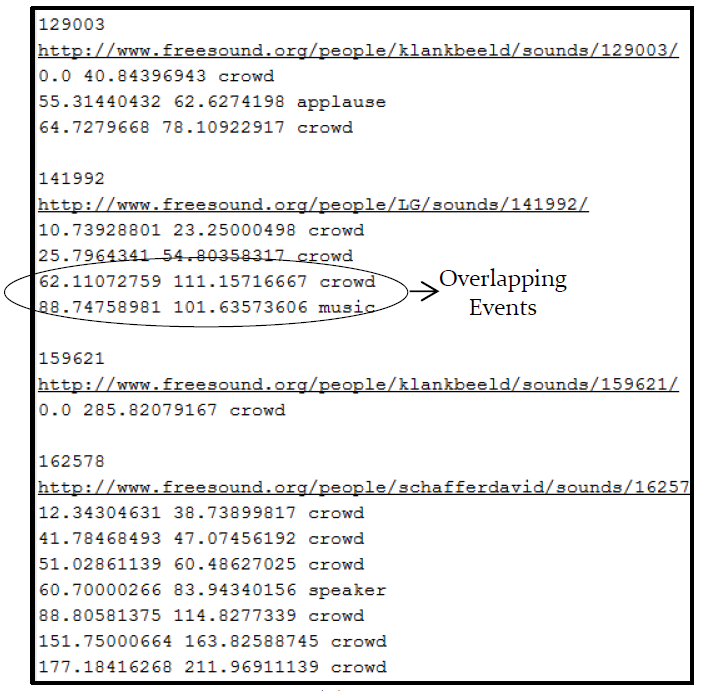
\includegraphics[width=0.8\columnwidth]{sample_annotation_db2} 
\caption[Sample annotation for dataset-II]{Sample annotation for dataset-II}
\label{fig:sample_annotation_db2} 
\end{figure}

Originally, as described in \cite{kons2013audio}, this dataset had 84 audio recordings (228 minutes of data). But, we could procure only 69 of those audio files because the other 15 were taken off from the website. Among these 15 files, as observed from the available annotations, most of the content belonged to the 'Music' class. More precisely, 20 out of the 84 audio recordings had 'Music' as an audio event in them. Among these 20 recordings, 6 of them were almost entirely 'music' sounds and all 6 of these were among the recordings that could not be procured. Hence, there was a significant loss of data belonging to a certain audio class. In our experiments, to compensate for this loss, we also tried adding 6 randomly chosen musical recordings from the \textsl{freesound} website with almost same total duration of data as was lost. For completeness, we present our results both with and without the extra 'Music' files.

The 69 recordings that we procured were of variable duration and as per \cite{kons2013audio}, we sliced out audio segments of a fixed length (5 seconds) with an overlap of 2.5 seconds between segments, from these recordings. This gave us approximately 4200 audio segments. Each of these segments were then treated as one training data instance for our machine learning models. The audio event labels for these segments were decided on the basis of the following criterion- in a given audio segment of 5 seconds, whichever audio event classes are labeled in the annotations within that 5 second duration, are to be considered as the audio event class labels for that audio segment. For example if there is a segment that begins from 0 sec and ends at 5 secs in the parent recording. And if in the annotations, we have 'Crowd' annotated from 2 sec to 4 sec, 'Applause' annotated from 6 sec to 12 sec, and 'Traffic annotated from 4 sec to 8 sec, then the audio segment will have the following labeled classes: 'Crowd' and 'Traffic', because both of them are (partly or wholly) present in that segment.

Despite of having the 6 audio event classes initially, we did all our experiments with just 4 audio event classes: (i)Crowd, (ii)Applause, (iii)Music, and (iv)Traffic. This is because the baseline results for this dataset published in \cite{kons2013audio} report the results for only these 4 classes. Hence, to make a comparison we report our results as well for just these 4 classes. Further details about the dataset can be found in \cite{kons2013audio}

\subsection{Dataset-III}

\begin{table}[!htb]
\caption[CHiME Dataset - Audio Classes]{CHiME Dataset - Audio Classes}
\label{tab:audio_classes_db3_bkg}
\centering
\begin{tabular}{ccc}
\toprule
Label & Description  \\
\midrule
c	& Child speech\\
m	& Adult male speech\\
f & Adult female speech\\
v 	& Video game/TV\\
p & Percussive sounds, e.g. crash, bang, knock, footsteps\\
b & Broadband noise, e.g. household appliances\\
o & Other identifiable sounds\\
\bottomrule 
\end{tabular}
\end{table}

The third and last dataset we worked on is another publicly available dataset, know as the CHiME-Home\footnote{https://archive.org/details/chime-home}(Computational Hearing in  Multisource Environments) dataset. As the name suggests, this dataset has sounds coming from multiple sources, hence it is a polyphonic audio events dataset. The recordings are confined to a home environment and in fact all the recordings of this dataset are made at the same place inside a house. 

This dataset has a total of 6.8 hours of audio recordings with 7 possible audio event classes as listed in table~\ref{tab:audio_classes_db3_bkg}. Similar to the previous two datasets, each audio recording here is of fixed length (4 seconds). Actually the original recordings are sliced down to these fixed length excerpts (non-overlapping) and there are 4378 such audio excerptsin the dataset. The audio event class label for each excerpt is a set of the mentioned audio classes, with the set having one or many of them. More details about the dataset can be found at \cite{christensen2010chime}. The baseline results for this dataset using Gaussian Mixture Model along with the implementation details are available at \cite{foster2015chime}. We also compare the results of our model on this dataset to the baseline results as a part of our work.
